\documentclass[10pt]{extarticle}
\title{}
\author{}
\date{}
\usepackage[shortlabels]{enumitem}


%paper setup
\usepackage{geometry}
\geometry{letterpaper, portrait, margin=1in}
\usepackage{fancyhdr}
% sans serif font:
\usepackage{cmbright}
%symbols
\usepackage{amsmath}
\usepackage{bigints}
\usepackage{amssymb}
\usepackage{amsthm}
\usepackage{mathtools}
\usepackage{bbm}
\usepackage[colorlinks=true,urlcolor=blue]{hyperref}
\usepackage{gensymb}
\usepackage{multirow,array}
\usepackage{multicol}

\newtheorem*{remark}{Remark}
\usepackage[T1]{fontenc}
\usepackage[utf8]{inputenc}

%chemistry stuff
%\usepackage[version=4]{mhchem}
%\usepackage{chemfig}

%plotting
\usepackage{pgfplots}
\usepackage{tikz}
\tikzset{middleweight/.style={pos = 0.5}}
%\tikzset{weight/.style={pos = 0.5, fill = white}}
%\tikzset{lateweight/.style={pos = 0.75, fill = white}}
%\tikzset{earlyweight/.style={pos = 0.25, fill=white}}

%\usepackage{natbib}

%graphics stuff
\usepackage{graphicx}
\graphicspath{ {./images/} }
\usepackage[style=numeric, backend=biber]{biblatex} % Use the numeric style for Vancouver
\addbibresource{the_bibliography.bib}
%code stuff
%when using minted, make sure to add the -shell-escape flag
%you can use lstlisting if you don't want to use minted
%\usepackage{minted}
%\usemintedstyle{pastie}
%\newminted[javacode]{java}{frame=lines,framesep=2mm,linenos=true,fontsize=\footnotesize,tabsize=3,autogobble,}
%\newminted[cppcode]{cpp}{frame=lines,framesep=2mm,linenos=true,fontsize=\footnotesize,tabsize=3,autogobble,}

%\usepackage{listings}
%\usepackage{color}
%\definecolor{dkgreen}{rgb}{0,0.6,0}
%\definecolor{gray}{rgb}{0.5,0.5,0.5}
%\definecolor{mauve}{rgb}{0.58,0,0.82}
%
%\lstset{frame=tb,
%	language=Java,
%	aboveskip=3mm,
%	belowskip=3mm,
%	showstringspaces=false,
%	columns=flexible,
%	basicstyle={\small\ttfamily},
%	numbers=none,
%	numberstyle=\tiny\color{gray},
%	keywordstyle=\color{blue},
%	commentstyle=\color{dkgreen},
%	stringstyle=\color{mauve},
%	breaklines=true,
%	breakatwhitespace=true,
%	tabsize=3
%}
% text + color boxes
\renewcommand{\mathbf}[1]{\mathbbm{#1}}
\usepackage[most]{tcolorbox}
\tcbuselibrary{breakable}
\tcbuselibrary{skins}
\newtcolorbox{problem}[1]{colback=white,enhanced,title={\small #1},
          attach boxed title to top center=
{yshift=-\tcboxedtitleheight/2},
boxed title style={size=small,colback=black!60!white}, sharp corners, breakable}
%including PDFs
%\usepackage{pdfpages}
\setlength{\parindent}{0pt}
\usepackage{cancel}
\pagestyle{fancy}
\fancyhf{}
\rhead{Avinash Iyer}
\lhead{Economics of Education: Class Notes}
\newcommand{\card}{\text{card}}
\newcommand{\ran}{\text{ran}}
\newcommand{\N}{\mathbbm{N}}
\newcommand{\Q}{\mathbbm{Q}}
\newcommand{\Z}{\mathbbm{Z}}
\newcommand{\R}{\mathbbm{R}}
\setcounter{secnumdepth}{0}
\begin{document}
\section{Introduction}%
Education is one of the largest sectors in the economy, and thus can be studied from a large amount of angles.
\begin{itemize}
  \item Early Childhood Education (beyond just ``being watched'')
  \item Elementary/Secondary School
  \item Postsecondary Education
\end{itemize}
Education can be studied from a lot of angles:
\begin{description}
  \item[Micro:] Applying theories of labor economics and consumer theory to education.
  \item[Econometrics:] Use data to analyze educational policies.
  \item[Macro:] Investigate global demand for education-as-a-commodity.
\end{description}
\subsection{Education System Basics}%
\begin{description}
  \item[Returns to Education:] There is a large return to education; those with a high school education tend to make far less than those with a bachelor's degree and up. Perceived value of being more education in private or public market.
  \item[Labor Market Outcomes:] The more educated you are, the more likely to have a job; unemployment rates for high school graduates are higher than unemployment rates for college graduates.
  \item[Public Spending:] Approximately 5--6\% of GDP is spent on education in most OECD countries.
  \item[Funding Structure:] Public schools are primarily funded through state and local governments --- property taxes the largest source of funding for education, but federal government has started to fund more schools in recent years.
  \item[Growth of Education over Time:] Claudia Goldin's 1993 paper ``The Human-Capital Century and American Leadership'' shows that the 20th century was really the century of greater and greater access and attainment in education.
\end{description}
\section{Why Do We Get Educated?}%
\subsection{Human Capital}%
  \begin{description}
    \item[What is human capital?]\hfill
      \begin{itemize}
        \item Labor. 
        \item Complexity or efficiency of work.
      \end{itemize}
    \item[How does human capital differ from capital?]\hfill
      \begin{itemize}
        \item Less static.
        \item Differential depreciation --- potential for appreciation (people can skill up).
        \item Higher variance.
        \item Unionization/collective bargaining.
        \item Idea generation.
        \item Potentially greater mobility.
        \item Returns to human capital come in the form of wages --- human capital is owned by the human that holds it.
        \item Cannot be collateralized.
        \item Divisibility (or lack thereof).
      \end{itemize}
  \end{description}
\subsection{Education: how much?}%
  \begin{description}
    \item[Discrete Model:] To college or not?
      \begin{itemize}
        \item Direct costs: tuition, room and board.
        \item Indirect costs: foregone earnings.
        \item Returns: expected future earnings (requires college degree or not). 
      \end{itemize}
      We will assume that ``college'' is period 1, and college grads earn more post-college, and there is a discount rate $r$. 
      \begin{center}
        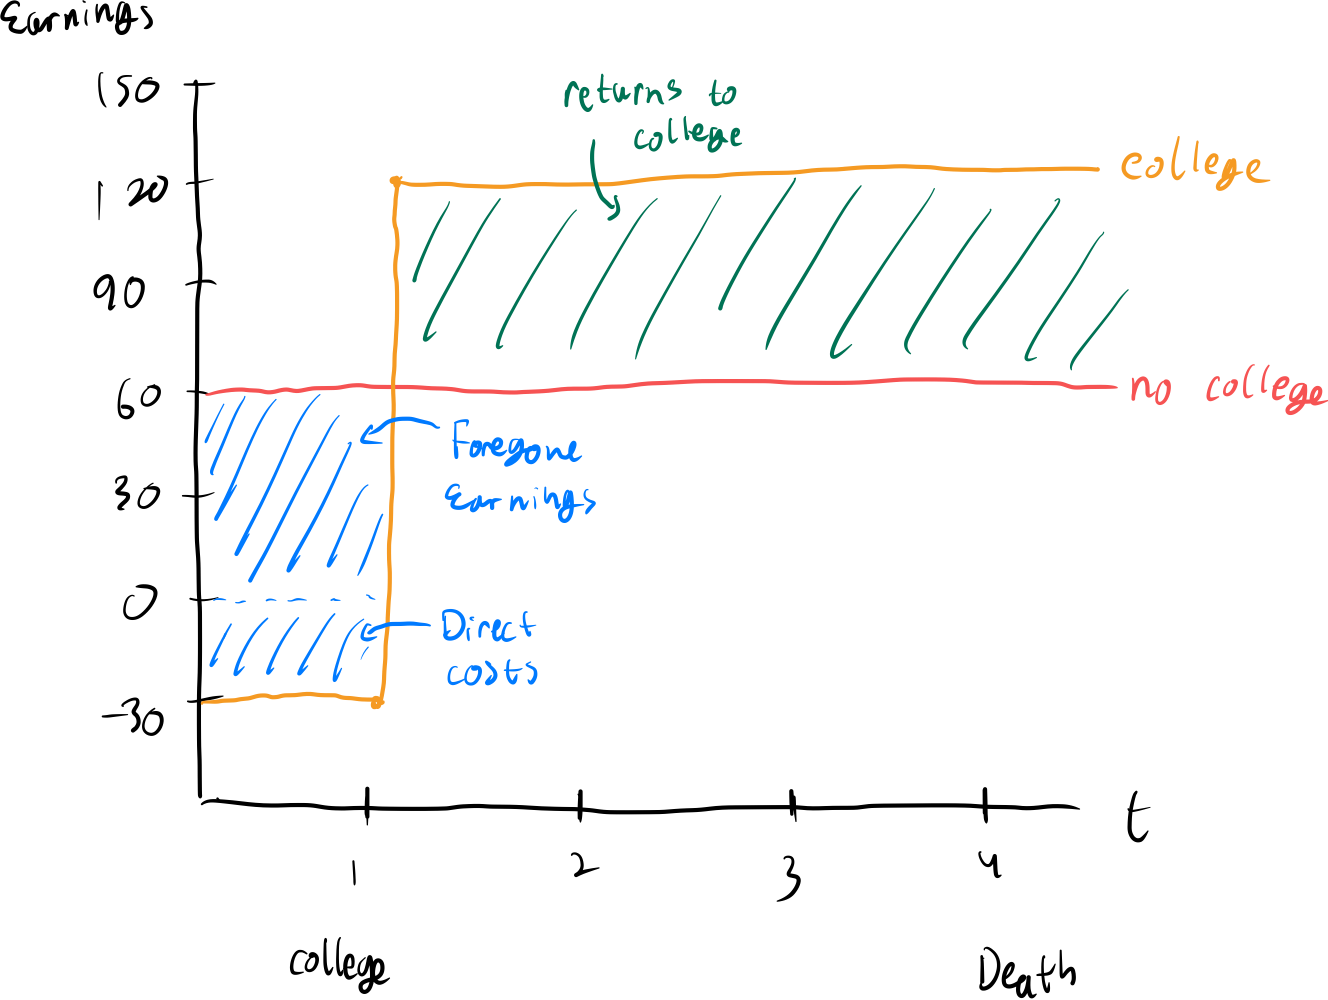
\includegraphics[width=10cm]{images/discrete_education_model.png}
      \end{center}
      The discount rate of \$100 in $t>0$ periods is worth $\frac{100}{(1+r)^t}$ in period $0$ (aka today).\\

      We generally think about $r$ in terms of the interest rate --- money today is worth more than money in the future due to the ability to invest.\\

      The \textit{present value} of a stream of money is found as follows:
      \begin{align*}
        \text{PV} &= \frac{100}{(1+r)} + \frac{100}{(1+r)^2} + \cdots + \frac{100}{(1+r)^n}\\
                  &= \sum_{t=1}^{n} \frac{100}{(1+r)^t} \tag*{$(1)$}\\
        (1+r)\text{PV} &= 100 + \frac{100}{(1+r)} + \cdots + \frac{100}{(1+r)^{n-1}}\\
                       &= 100 + \sum_{t=1}^{n-1} \frac{100}{(1+r)^t} \tag*{$(2)$}\\
        (1+r)\text{PV} - \text{PV} &= 100 + \sum_{t=1}^{n-1}\frac{100}{(1+r)^t} - \sum_{t=1}^{n-1}\frac{100}{(1+r)^t} - \frac{100}{(1+r)^n}\tag*{$(2)-(1)$}\\
        r\text{PV} &= 100 - \frac{100}{(1+r)^n}\\
        \text{PV} &= \frac{100}{r}\left(1-\frac{100}{(1+r)^n}\right)
      \end{align*}
      As $n$ becomes larger, then the PV of the asset is larger. For example, if $n = 40$, $Y = 60,000$, and $r = 0.05$, then the PV of this revenue stream is approximately \$1 million.\\

      Bringing this to the model, where $F$ denotes direct tuition cost, $Y_0$ denotes earnings with no schooling, and $Y_S$ denotes earnings with schooling (where school occurs in period $1$).
      \begin{align*}
        \text{PV}_{0} &= \frac{Y_0}{(1+r)} + \frac{Y_0}{(1+r)^2} + \cdots + \frac{Y_0}{(1+r)^n}\\
        \text{PV}_{S} &= -F + \frac{Y_S}{(1+r)^2} + \cdots + \frac{Y_S}{(1+r)^n}\\
        \text{NPV}_{S} &= \text{PV}_{S} - \text{PV}_{0}\\
                       &= \underbrace{-F - \frac{Y_0}{(1+r)}}_{\small\text{Cost}} + \underbrace{\sum_{t=2}^{n}\frac{Y_S - Y_0}{(1+r)^t}}_{\small\text{Benefit}}\\
                       &= -F-\frac{Y_0}{1+r} + \frac{Y_S-Y_0}{r}\left(1-\frac{1}{(1+r)}\right)\frac{1}{1+r}
      \end{align*}
      To find if education is worth it, we calculate if $\text{NPV}_{S} > 0$.
    \item[Continuous Model (or Mincer Model):] To take an extra year of education or not?
      \begin{itemize}
        \item $S$ is a discrete, integer choice (denoting a year of education).
        \item $Y_S$ is salary after schooling for $S$ years.
        \item There are zero direct costs of school.
        \item Years in labor force, $K$, are equivalent regardless of $S$.
      \end{itemize}
      We choose $S$ where marginal benefit is equal to marginal cost.
      \begin{align*}
        \text{PV}_{S} &= \text{PV}_{S+1}\\
        \sum_{t=1}^{K}\frac{Y_S}{(1+r)^t} &= \sum_{t=2}^{K+1}\frac{Y_{S+1}}{(1+r)^t}\\
        \frac{Y_S}{r}\left(1-\frac{1}{(1+r)^K}\right) &= \frac{Y_{S+1}}{r}\left(1-\frac{1}{(1+r)^K}\right)\frac{1}{1+r}\\
        Y_S &= Y_{S+1}\frac{1}{1+r}\\
        1+r &= \frac{Y_{S+1}}{Y_S}
      \end{align*}
      We choose school until the marginal rate of return is equal to the discount rate.
  \end{description}
  \textbf{Housekeeping, January 30:} Schedule for discussion and presentation is located \href{https://docs.google.com/document/d/1uy96HLNuZVGlrT8oiC49i3M6p2E57fopxGwizHv4_Hs/edit}{at this link}, and the guidelines for classroom activities are located \href{https://docs.google.com/document/d/1tnPmI21LJLdKblCUbuFMuDGobuAz2IOaineH_I4BTFg/edit}{at this link}.
  \subsection{Educational Landscape}%
  The human capital system consists of a number of components.
  \begin{itemize}
    \item Trade, technical, and vocational education (generally falls under post-secondary education)
    \item Early childhood education --- Ages 6 weeks--5, includes day care and pre-K
    \item Primary education --- Ages 5--12, Grades K--5/6
    \item Secondary education --- Ages 12--18, Grades 6--12
    \item Post-secondary education --- two year/community college, four year college
    \item Graduate education --- profession-oriented (MBA, JD), research-oriented (master's, PhD), certification (CPA, CFA, actuarial credentialing)
    \item Adult education (GED, college)
  \end{itemize}
  In primary and secondary education, primary choice facing consumers of education is between public and private education.
  \subsection{Human Capital Model: Choice of Schooling Quantity}%
  The human capital model indicates that consumers of education choose their amount of schooling, $S$, based on the following factors:
  \begin{itemize}
    \item Discrete: $Y_S$ (income from having been schooled) vs $Y_0$ (income without schooling)
    \item Continuous: $\frac{Y_{S+1}}{Y_S}$ (marginal rate of return from schooling)
    \item $F$ (the cost of schooling)
    \item $r$ (discount rate)
  \end{itemize}
  However, this leads us to ask an important question --- why might $S$ differ?
  \begin{itemize}
    \item Differing (marginal) rates of return --- job-specific factors, overqualification, ability, quality of education
    \item Different cost of education --- borrowing, aid, credit constraints
      \begin{description}
        \small
        \item[Comment:] Credit constraints increase exponentially as quantity of schooling increases.
      \end{description}
  \end{itemize}
  A model of credit constraints' effects on choices of education can be seen as follows:
  \begin{center}
    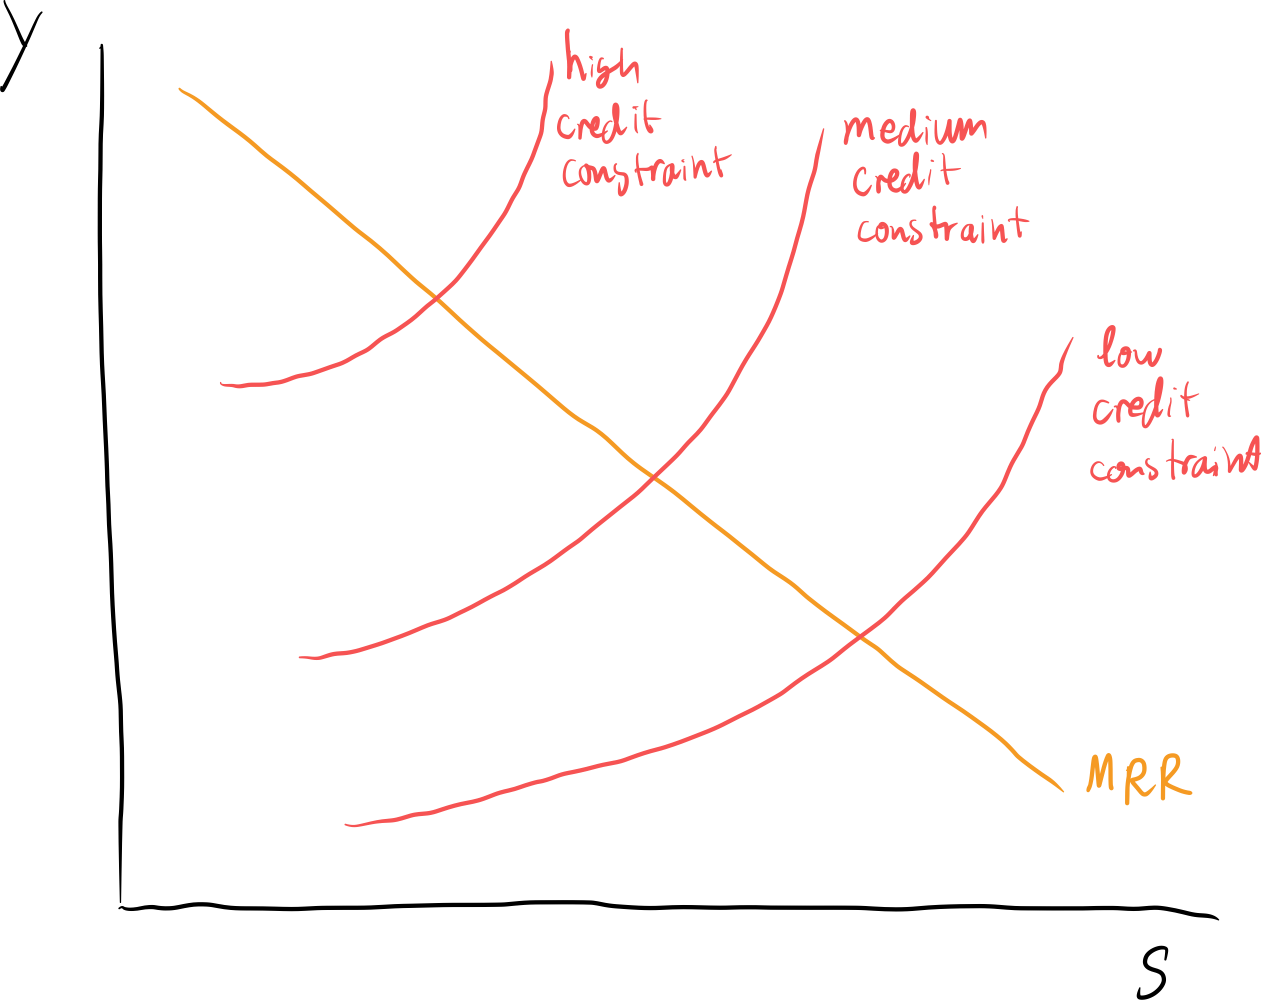
\includegraphics[width=10cm]{images/credit_constraints.png}
  \end{center}
  Broadly speaking, if $S$ differs because of marginal rate of return, then subsidies may be inefficient --- subsidies will cause inefficient excess schooling.\\

  However, if $S$ differs because of cost, then subsidies improve overall output and efficiency.
  \subsection{Signaling}%
  The basic idea behind the human capital model is that by getting more educated, you become smarter and have a higher rate of return --- regardless of whether or not you get a degree. Now, we will discuss a model where schooling does not indicate one's level of smartness.
  \begin{description}
    \item[Assumptions:]\hfill
      \begin{enumerate}[(1)]
        \item No human capital accrued at school.
        \item Two types of workers: low ability ($L$) of proportion $p$ with productivity $1$ and high ability ($H$) of $1-p$ with productivity $2$.
        \item Cost of education is lower for type $H$. For type $L$, the cost of education is $c$, and for type $H$ the cost of education is $c/2$.
        \item Generic employer who, if they distinguish $H$ and $L$, pay marginal benefit --- wage to $L$ is $1$, wage to $H$ is $2$.
        \item If the employer cannot distinguish between $H$ and $L$, then they pay the expected marginal benefit, $(1-p)(2) + (p)(1) = 2-p$.
      \end{enumerate}
    \item[Game Play:] \hfill
      \begin{itemize}
        \item Employer forms belief $w(S)$ about the worker productivity
        \item Employer sets $w(S)$
        \item Workers observe $w(S)$ and decide on $S$
        \item Workers are hired and firms observe their productivity
      \end{itemize}
    \item[Types of Equilibria:]\hfill
      \begin{itemize}
        \item Separating equilibrium: a situation where $H$ chooses education and $L$ does not choose education. In this case, education serves as a pure signal of high productivity --- there is no separating equilibrium where $H$ chooses no education and $L$ chooses education.
        \item Pooling equilibrium: all workers choose education, and the employer cannot differentiate, meaning the employer pays $2-p$ to all workers.
      \end{itemize}
    \item[Finding a Separating Equilibrium:] We assume that there is a separating equilibrium --- $H$ chooses $S=1$ and $L$ chooses $S=0$. Then, the employer forms beliefs to set a wage structure as follows:
      \begin{align*}
        w(S) &= \begin{cases}
          2 & S=1\\
          1 & S=0
        \end{cases}.
      \end{align*}
      In order to be an equilibrium, both $H$ and $L$ types need to have an incentive not to deviate.
      \begin{itemize}
        \item $H$ Type Equilibrium Condition: Return to education is higher than return to non-education.
          \begin{align*}
            2 - \frac{c}{2} &> 1\\
            c &< 2
          \end{align*}
        \item $L$ Type Equilibrium Condition: Return to non-education is higher than return to education.
          \begin{align*}
            1 &> 2-c\\
            c &> 1
          \end{align*}
      \end{itemize}
      Therefore, if $c\in (1,2)$, we can find a separating equilibrium.
    \item[Finding a Pooling Equilibrium:] We assume that there is a pooling equilibrium where all players are educated --- $H$ chooses $S = 1$ and $L$ chooses $S = 1$. Then, the employer forms beliefs to set a wage structure as follows:
      \begin{align*}
        w(S) &= \begin{cases}
          2-p & S = 1\\
          1 & S = 0
        \end{cases}
      \end{align*}
      In order to be an equilibrium, both $H$ and $L$ types need to have an incentive not to deviate.
      \begin{itemize}
        \item $H$ type equilibrium Condition: Return to education is higher than return to non-education.
          \begin{align*}
            (2-p)-\frac{c}{2} &> 1\\
            c &< 2-2p
          \end{align*}
        \item $L$ type equilibrium condition: Return to education is higher than return to non-education.
          \begin{align*}
            (2-p)-c &> 1\\
            c &< 1-p
          \end{align*}
      \end{itemize}
      Therefore, so long as $c < 1-p$, both types of employees will choose education over non-education. Essentially, if the cost of education is very low, then everyone will choose education.\\

      Working through a similar set of logic, we can also find a sufficient $c$ such that everyone chooses no education.
      \begin{align*}
        w(S) &= \begin{cases}
          2-p & S=0\\
          2 & S=1
        \end{cases},
      \end{align*}
       if $c > 2p $. Notice that both of these pooling equilibria are more likely to exist the higher proportion of $H$ types.
  \end{description}
  \subsubsection{Signal vs Index}%
  \begin{itemize}
    \item Signal: implicit assurance of skill or quality, chosen by worker, not readily apparent. Examples include education levels.
    \item Index: worker cannot control said assurance of skill or quality, but predetermined, generally a source of discrimination. Examples include disability, race, gender, and age.
  \end{itemize}
  The signaling model starts with employers offering different wages based on a signal --- the signal is something a worker has some level of control.\\

  However, the signaling model could also be thought of as an indexing model (by varying parameters $p$ and $c$ while equalizing productivity). Essentially, the signaling model is about a legal form of discrimination (education-based discrimination), but we can apply it to illegal forms of discrimination.
  \subsection{Human Capital and Signaling Model: Features}%
  \begin{center}
    \renewcommand{\arraystretch}{1.5}
    \begin{tabular}{m{0.2\textwidth}|m{0.2\textwidth}|m{0.2\textwidth}}
      Human Capital & Both Models & Signaling Model\\
      \hline
      positive externalities & inequality & pure private returns\\
      education is efficient & & education is inefficient
    \end{tabular}
  \end{center}
  \section{Claudia Goldin: The Human-Capital Century}%
  \begin{itemize}
    \item The 20th century was the century where people became educated --- early on, few people even had a primary education, but now, the vast majority of people obtain secondary school.
    \item Education is democratic.
      \begin{itemize}
        \item Democracy is a government by the people, for the people.
        \item Power is not vested by God or inherent in blood, but governance comes from the consent of the governed.
        \item Public demand for education leads to more education being delivered.
        \item Education provides both skills and time to create better citizens.
      \end{itemize}
    \item Virtues: egalitarianism, forgiveness (possibly changing), separation of church and state.
    \item Primary education was very common across the rich world, but secondary education was far more common in the United States than other countries.
    \item Specifically, American secondary education was about \textit{general} education (algebra, writing, reading comprehension, etc.), not merely vocational or technical training. The European system is much more heavily tracked.
    \item Idea that one would spend years 10--18 in education began in the United States. Adults were better able to establish themselves in the new economy, and the underlying structures were exported to the rest of the United States.
    \item European systems developed out of monarchy/aristocracy, leading to deterministic ideas of the demands of the economy.
    \item Decentralized American education system --- curriculum followed the economy, rather than determined for the economy.
    \item The standards for general education developed around a pure method of approach towards problems.
    \item Rise of large corporations generated large need for management, idea generation, communication --- had to do HR, accounting, etc. at a scale never seen before. Skills were meant to be portable and transferable, which the decentralized American education system satisfied the demand for.
  \end{itemize}
  \section{Understanding Causality}%
  When discussing questions in economics, there are two basic approaches:
  \begin{itemize}
    \item Theory: models (as discussed in our model of human capital and the signaling model).
    \item Empirics: using data to understand the dynamics of the world.
  \end{itemize}
  For example, we may want to understand the impact of a good teacher in the role of educational success through different measures:
  \begin{itemize}
    \item Pass rates or graduation rates.
    \item College entrance rates.
    \item Test scores.
    \item Earnings.
  \end{itemize}
  We can think of each of these as our $Y_i$, our outcome variable of interest. At the same time, we have to measure the quality of a teacher, $X_i$, through different mechanisms:
  \begin{itemize}
    \item Education
    \item Course Evaluations (with adequate controls for race and gender)
    \item Subject
  \end{itemize}
  \subsection{Defining Causality}%
  The impact of variable $A$ \textit{causally} affects variable $B$ as the change in $B$ if $A$, and only $A$, is altered. Causality is usually defined using a counterfactual.\\

  In the case of education, for $Y_i$, student $i$'s outcome, with $Y_{1i}$ for an outcome for a student with a good teacher and $Y_{0i}$ for a student with a bad teacher. We define $D_i$, our dummy variable, as $1$ if the teacher is good and $0$ if the teacher is bad.
  \begin{align*}
    Y_i &= Y_{0i} + D_i\underbrace{(Y_{1i} - Y_{0i})}_{\text{treatment effect}}.
  \end{align*}
  \subsection{Potential Outcomes Framework}%
  \begin{itemize}
    \item What does a researcher observe? We assume $N>1$. In this case, 
  \end{itemize}
  \begin{align*}
    E(Y_{1i}|D_i=1) - E(Y_{0i}|D_i=0) &= \text{ observed difference of $D_i = 1$ }\\
                                      &= \overbrace{E(Y_{1i}|D_i = 1) - \underbrace{E(Y_{0i}|D_i=1)}_{\text{counterfactual}}}^{\text{Average Treatment Effect (impact of good teacher)}}\\
                                      &+ \overbrace{\underbrace{E(Y_{0i}|D_i=1)}_{\text{counterfactual}} - E(Y_{0i}|D_i=0)}^{\text{selection bias}}
  \end{align*}
  Therefore, we can see that the observed difference is a function of treatment and selection bias. The most difficult part of empirical research is finding situations where selection bias is as close to zero as possible.\\

  In regression analysis, we might have the model that states
  \begin{align*}
    \text{score}_i &= \beta_0 + \beta_1\text{TeacherQuality}_i + \varepsilon_i.
  \end{align*}
  \begin{center}
    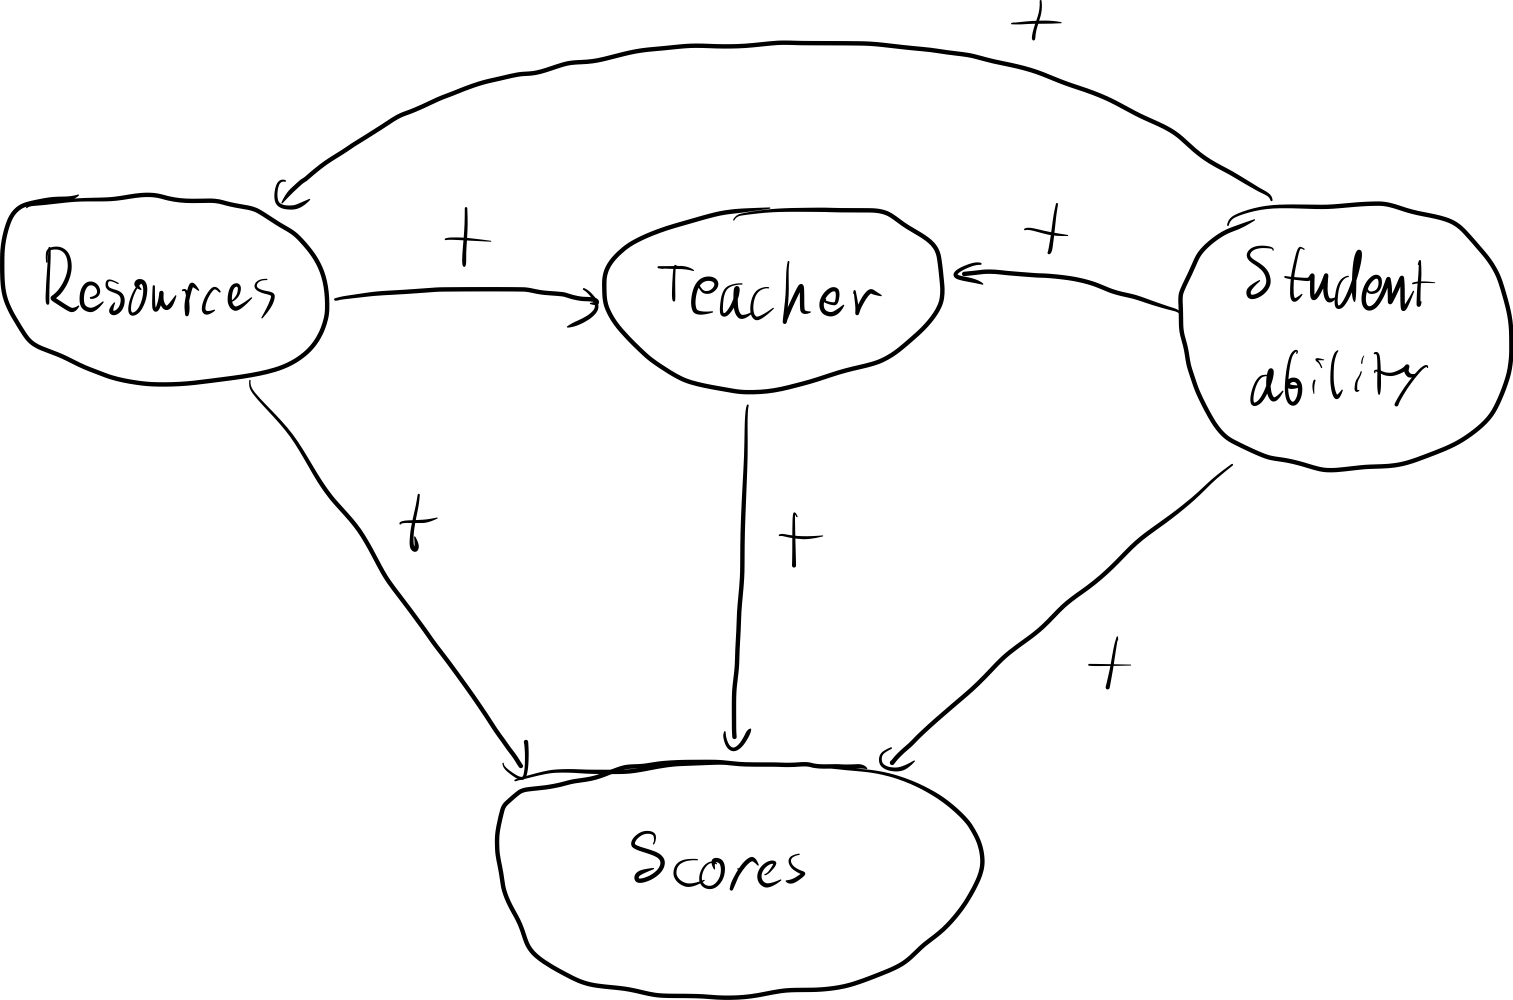
\includegraphics[width=10cm]{images/test_score_variables.png}
  \end{center}
  Suppose that teachers matter --- even then, there are other variables, such as resources or intrinsic ability. The diagram depicts the various ways that selection bias can create positive correlation.\\

  In this case, $\hat{\beta_1}$ will be biased by selection. This is known as omitted variable bias, and violates the principle that $\text{Cov}(X,\varepsilon) = 0$.\\

  To resolve this, we may update our regression model to control for the omitted variable of resources, denoted $Z$.
  \begin{align*}
    \text{score}_{i} &= \beta_0 + \beta_1\text{TeacherQuality}_i + \beta_2\text{Resources}_i + \varepsilon_i\\
    \text{observed effect} &= E(Y_{1i}|D_i=1,Z) - E(Y_{0i}|D_{i}=1,Z) + \underbrace{E(Y_{0i}|D_i=1,Z) - E(Y_{0i}|D_i=0,Z)}_{\text{selection bias}}.
  \end{align*}
  However this still leaves out other omitted variables (such as parental involvement). As we add more control variables, selection bias should reduce. All these control variables exist to mitigate selection bias and make a non-experimental setting as close to an experiment as possible.\\

  There are a few major ways to identify causality:
  \begin{enumerate}[(1)]
    \item Experiments
    \item Instrumental Variables
    \item Difference-in-difference
    \item Regression discontinuity
    \item Panel data
  \end{enumerate}
  \subsection{Experiments}%
  The ``cleanest'' way to 
  \begin{itemize}
    \item Identify a Target Population.
    \item Randomize Population.
      \begin{itemize}
        \item Treatment group experiences condition.
        \item Control group does not experience condition.
      \end{itemize}
    \item Experiments have the following desirable properties:
      \begin{itemize}
        \item Internal Validity: $E(\varepsilon|X) = 0$ (error is uncorrelated with independent variable)
        \item Randomness
      \end{itemize}
    \item However, true randomness is difficult to attain. The ABCs of experiments also threaten internal validity.
      \begin{itemize}
        \item Attrition: individuals drop out of experiments.
        \item Balance: distribution of covariates may not be the same across groups.
        \item Compliance: not everyone assigned to a treatment may experience it.
      \end{itemize}
    \item There are also other limits:
      \begin{itemize}
        \item Feasibility: expense, time, or even full impossibility.
        \item Ethics: some experiments may pose ethical issues
        \item External validity: experiments may only provide insights to specific situations.
      \end{itemize}
    \item Threats to internal validity:
      \begin{itemize}
        \item Poor randomization
        \item Experimental contamination
        \item Response rate, compliance
        \item Attrition
      \end{itemize}
    \item Threats to external validity:
      \begin{itemize}
        \item Non-representative sample
        \item Treatment depends on experiment
        \item Excessive controls, Hawthorne effect
        \item Scalability
      \end{itemize}
  \end{itemize}
  Many experiments in the economic literature occur through lotteries.
  \begin{itemize}
    \item Project Star: randomly assigned students to teachers and class sizes.
    \item Perry Preschool: balanced lottery for access to early childhood education.
    \item Expanding Opportunities Project: lottery for access to mentoring for high school students and college resources.
  \end{itemize}
  \subsection{Carrell et al.: A's from Zzzz's? The Causal Effect of School Start Time on the Academic Achievement of Adolescents}%
  \begin{itemize}
    \item Why might we be skeptical of a paper without the controlled environment inherent at USAFA?
      \begin{itemize}
        \item Student choice.
        \item Grading style.
        \item Teacher quality, teaching style, teacher tiredness, experience based on time period.
        \item Student selection into teachers.
        \item Commutes.
        \item Extracurriculars and physical fitness.
        \item Food and energy.
        \item Study habits.
        \item Circadian rhythm.
        \item Cheating.
        \item Day of week.
      \end{itemize}
    \item What is special about the USAFA?
      \begin{itemize}
        \item Common exam timings.
        \item Course difficulty held constant.
        \item Mandatory breakfast.
        \item Grading styles held constant.
        \item No choice in schedule.
        \item No commutes.
        \item Physical fitness requirements.
        \item No zero period classes.
        \item Teachers are randomized.
      \end{itemize}
      From a policy perspective, if the problem is time of day, then shifting schedules will do a lot of good. However, if the problem is being driven by sleep, then shifting time of day may not increase benefits all that much.
    \item How do they get to causality? Generally, we need variance in $X$ to find $\hat{\beta}_{1}$.
      \begin{itemize}
        \item Shifting of schedules.
        \item Block schedule that is not constant on day of week.
      \end{itemize}
    \item External Validity?
      \begin{itemize}
        \item The fact that attendees to the academy opt into the particular regimentation, and yet their outcomes for morning classes are so negative, suggests that the effects are actually larger than seen in the paper.
      \end{itemize}
  \end{itemize}
  \subsection{Quasi-Experimental Causality}%
  In the Carrell et al. paper, rather than an experiment, they used a ``good'' regression (essentially, a substantial set of randomization). However, now, we will examine three different methods of quasi-experimental causality.
  \begin{description}
    \item[Difference-in-difference:]\hfill
      \begin{itemize}
        \item Used in: analyzing results of natural experiments.
        \item Need: treatment variable, ``pre'' and ``post'' data on the same observations, two dummy variables and an interaction term. Control variable needs to be credible as a counterfactual.
        \item Can: provide credibly causal estimates that remove omitted variable bias, if used right.
        \item Example:
          \begin{itemize}
            \item Rosenwald initiative: some counties received money for school construction, others did not; counties that received money were similar to those that did not. Counties that got schools ended up with higher increase in literacy than those that did not receive schools. The treatment effect accounts for the gain in literacy \textit{relative to counterfactual.}
          \end{itemize}
        \item Benefit of difference-in-difference is that it's okay for the samples to be unbalanced. All we need is believing both groups were trending in the same direction, which is a weaker assumption, known as the parallel trends assumption.
      \end{itemize}
    \item[Instrumental Variables:] \hfill
      \begin{itemize}
        \item Used in: dealing with omitted variable bias.
        \item Require: fluke or randomness in source of causality that is not correlated with error.
        \item Example:
        \begin{itemize}
          \item Hurricanes in Puerto Rico caused schools to become more crowded close to the path of the hurricane.
          \item Use $Z_i$ to isolate part of class size that is only due to storm to obtain unbiased effect of class size on test scores.
        \end{itemize}
      \end{itemize}
    \item[Regression Discontinuity:]\hfill
      \begin{itemize}
        \item Arbitrary cutoff, hard or impossible to manipulate.
        \item Observations below cutoff do not receive a treatment, observations above cutoff do receive a treatment.
        \item Jump at the cutoff suggests credibly causal effect of treatment.
        \item Strong external validity.
        \item Examples:
          \begin{itemize}
            \item PSAT: hard to control whether under or over threshold of National Merit Scholarship. Results suggest effect of receiving money is quite positive.
            \item Head Start: based on Congress's design, the poverty line cutoff suggests we can examine results based on counties just below or above the cutoff.
          \end{itemize}
      \end{itemize}
  \end{description}
  \section{The Market for Education}%
  \begin{description}
    \item[Education productivity:] What, in our experience, has increased our education productivity?
      \begin{itemize}
        \item extracurriculars (sports, paper, clubs, etc.)
        \item peer pressure
        \item productive procrastination
        \item siblings
        \item jobs/internships (skills, selection, etc.)
        \item literacy
        \item food, recess
        \item problem sets and hands-on practice
        \item ``the grind''
        \item time management
      \end{itemize}
  \end{description}
  Today is effectively a recap of intermediate microeconomics, applying towards education concepts.
  \begin{description}
    \item[Supply:] Schools or teacher labor hours.
    \item[Demand:] Students.
    \item[Externalities:] Positive externalities? Negative externalities?
      \begin{itemize}
        \item Positive spillovers from higher education --- higher innovation, better functioning (political institutions), higher total factor productivity.
      \end{itemize}
    \item[Market Competition:] Cases for high vs. low market concentration.
      \begin{itemize}
        \item Some competition (public vs. private school).
        \item If one does not have the means to afford private school, often have one choice of school to send child to --- moving has high costs. Lots face a monopolistic market.
        \item Paradigm primarily applies toward primary education.
      \end{itemize}
    \item[Asymmetric Information:] Asymmetric information occurs when the supplier or demander of the education doesn't know the answer.
      \begin{itemize}
        \item Quality of school or teacher is often hard to measure.
        \item Schools may be terrible but that news may not be available to the students.
      \end{itemize}
    \item[Natural Monopolies:] Often lend themselves to government regulation.
      \begin{itemize}
        \item Electricity transmission: very high fixed cost, very low marginal cost.
        \item Education can also be thought of as a natural monopoly. Extremely expensive to develop a new school, but (relatively) low cost to enroll a new student. Transportation costs also increase the cost of switching.
      \end{itemize}
    \item[Economies of Scale:] Declining costs, increased returns to scale.
      \begin{itemize}
        \item Large public universities tend to spend much less per student than small colleges.
      \end{itemize}
    \item[Tracking or Stratifying:] different lanes or tracks, ones that aren't obtained early enough are closed off.
      \begin{itemize}
        \item Certain opportunities may be forever closed if you didn't obtain a certain math class in 7th grade.
        \item Higher education is a bit of a tracking system too.
        \item Tracking in education increases the older one is.
      \end{itemize}
    \item[Suppliers:]\hfill
      \begin{itemize}
        \item Public: state or local government.
        \item Private non-profit: parochial school, secular private schools.
        \item Private for-profit: most common for higher or adult education.
      \end{itemize}
    \item[Government Involvement:] Education is quite like the electricity or healthcare market --- asymmetric information, high costs to switching, extensive public involvement.
      \begin{itemize}
        \item Argument for public provision: positive externalities tend to be underfunded.
        \item Feature of public provision: subject to intervention (Brown v. Board, No Child Left Behind, Serrano v. Priest).
        \item Almost \$1 Trillion per year is spent by local and state governments on education, approximately \$200 billion per year is spent by the federal government, 50\% of which is spent on K--12 education. There has been a trend towards greater centralization of education finance.
      \end{itemize}
    \item[Inputs:]\hfill
      \begin{itemize}
        \item In micro, we have a utility function, $U(X_1,X_2)$.
        \item Demand for education: student production function.
        \item Supply for education: school production function.
        \item We will refer to a general education production function $y = f(x_1,x_2)$.\\

          We often assume that the production function is linear.
          \begin{align*}
            y_i = \beta_0 + \beta_1x_{1i} + \cdots + \beta_Kx_{Ki} + \varepsilon_i
          \end{align*}
          Linearity is not necessarily justifiable --- learning new things is hard, and certain skills (such as literacy) are often more valuable than other skills.\\

          We can also think of education production in a value-added model.
          \begin{align*}
            y_{it} - y_{it-1} = \beta_0 + \beta_1x_{1it} + \cdots + \beta_Kx_{Kit} + \varepsilon_{it}
          \end{align*}
          However, the problem with the input model is that we can't really measure or control a lot of these factors (like parental involvement).
      \end{itemize}
    \item[Outputs:]\hfill
      \begin{itemize}
        \item Students with education.
        \item Research.
      \end{itemize}
    \item[Hedonic Approach:]\hfill
      \begin{itemize}
        \item Price tells all (i.e., the value is what people are willing to pay).
        \item Valuation of non-market amenities is capitalized into the value of houses.
      \end{itemize}
    \item[Broad Trends on Education Spending:]\hfill
      \begin{itemize}
        \item America has roughly 18K school districts.
        \item There are approximately 50 million students, with average spending 18K per student, meaning we spend approximately 900 billion per year. 
        \item Education spending per pupil (in today's dollars) has expanded quite a bit since the 1940s.
        \item Reasons for increased spending:
          \begin{itemize}
            \item Infrastructure is more expensive.
            \item Human labor hours are more expensive.
            \item Economical to invest more in educating children.
          \end{itemize}
      \end{itemize}
    \item[Local Spending:] \hfill
      \begin{itemize}
        \item Tradition has been through property tax paid for by homeowners and businesses.
        \item Trend over time has been towards centralized public spending; federal sources make up approximately 10\% (mostly Title I and Free/Reduced Price Lunch). States tend to spend money through income tax, sales tax, excise tax, etc.
        \item Serrano v. Priest: fully local funding is unconstitutional. Between 1971 and 2010, 47 states adopted some form of finance equalization policy.
      \end{itemize}
    \item[Housekeeping:] Problem set 2 due February 27. Midterm 1 on February 29.
    \item[Forms of State Aid:] States support school funding through using state tax money to shift budget constraints in the locality ($B = X + R$).
      \begin{itemize}
        \item Block grant: unconditional funding for district. Assuming that education and other spending are normal goods (positive income effect)
          \begin{center}
            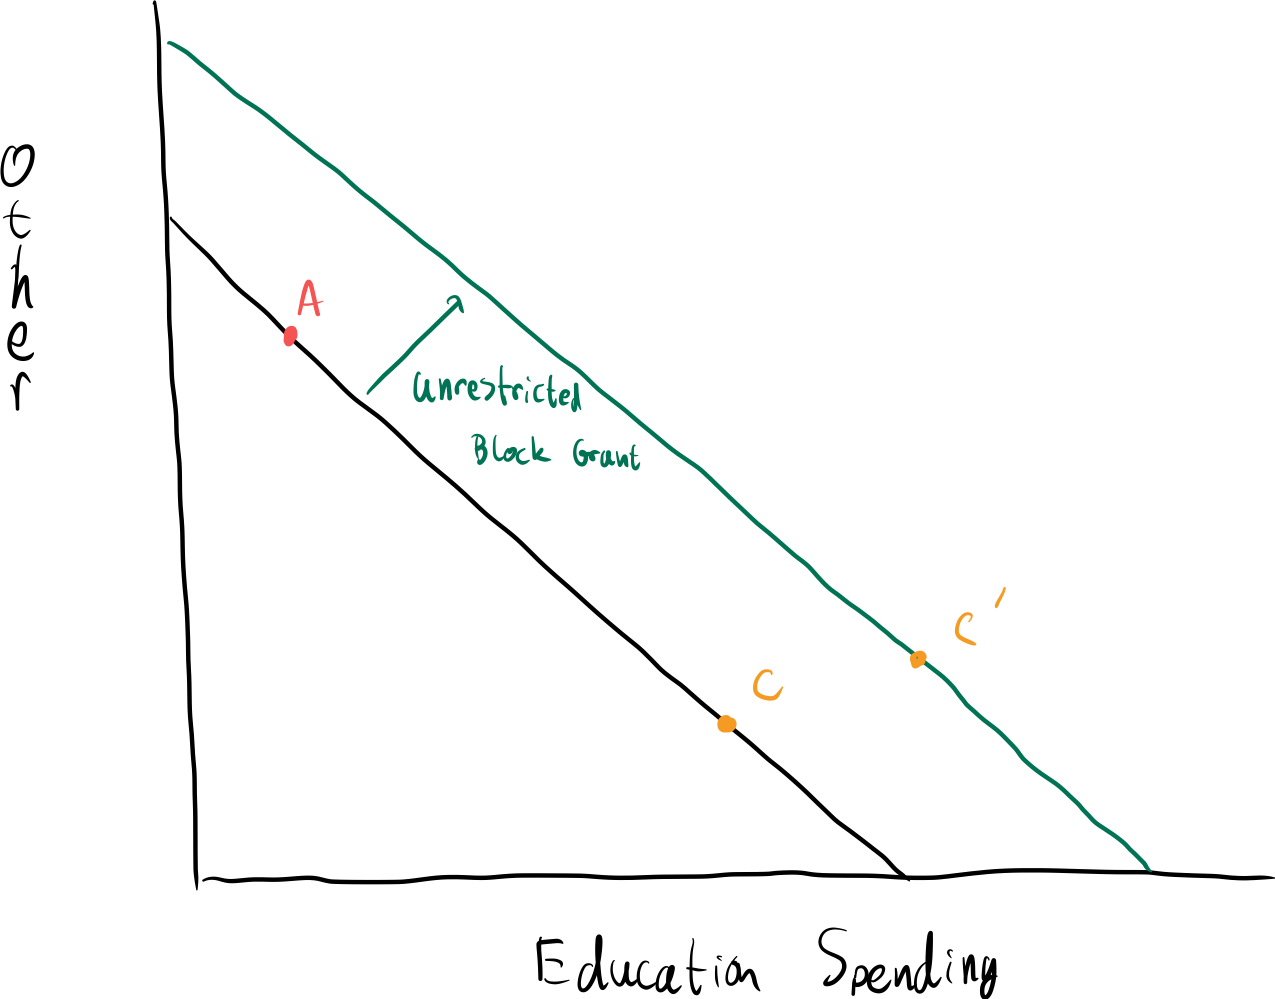
\includegraphics[width=10cm]{images/unrestricted_block_grant.png}
          \end{center}
        \item Conditional block grant: must be spent on education; $B = X + R + G$ if $R \geq G$.
          \begin{center}
            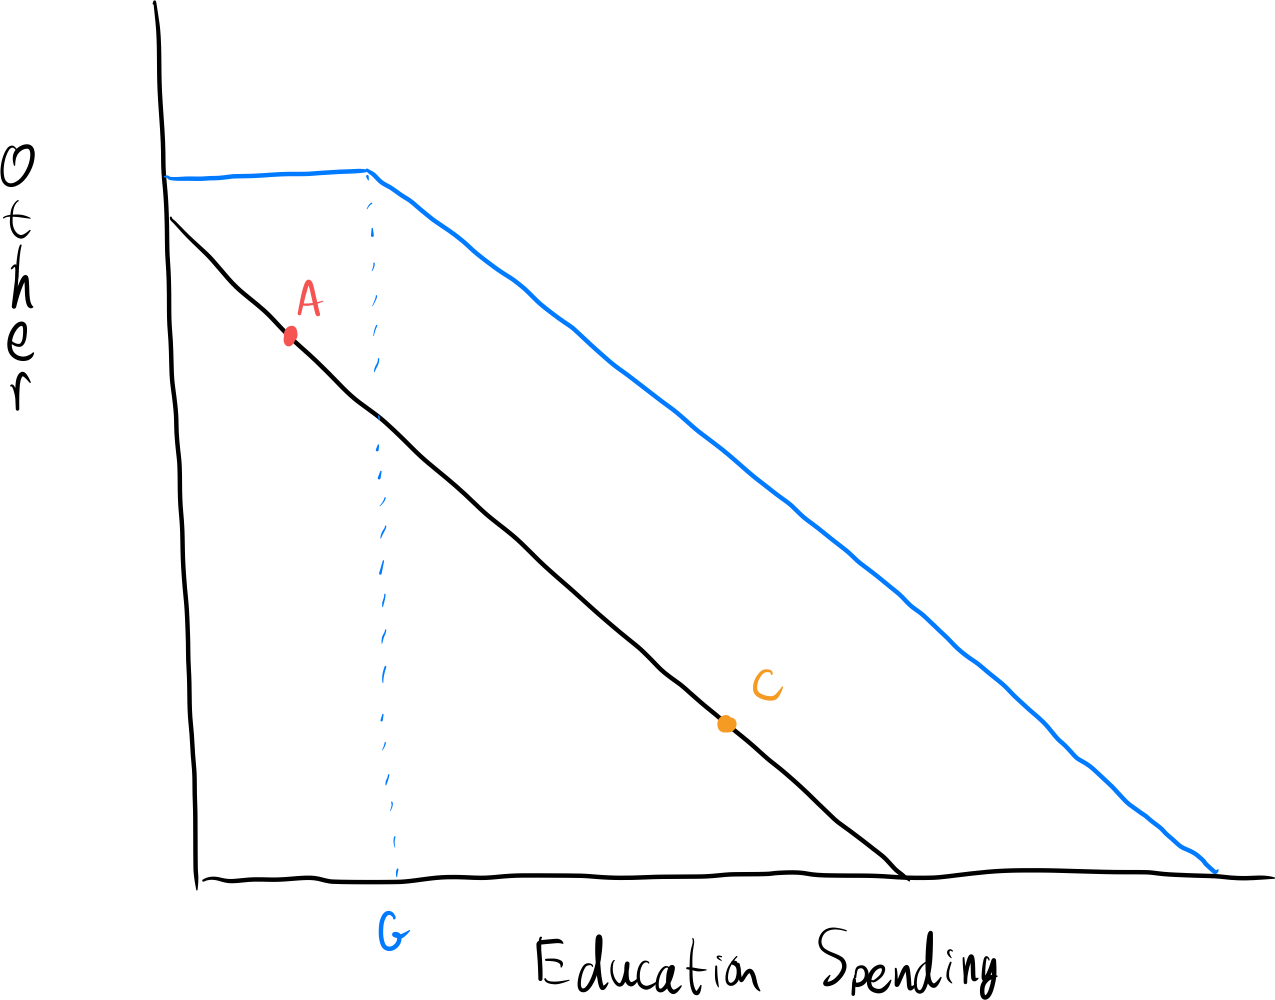
\includegraphics[width=10cm]{images/restricted_block_grant.png}
          \end{center}
        \item Matching grant: funding for district proportional to its spending. Reduces the price of education relative to other public spending. Substitution effect suggests more education spending, income effect suggests more other spending.
          \begin{center}
            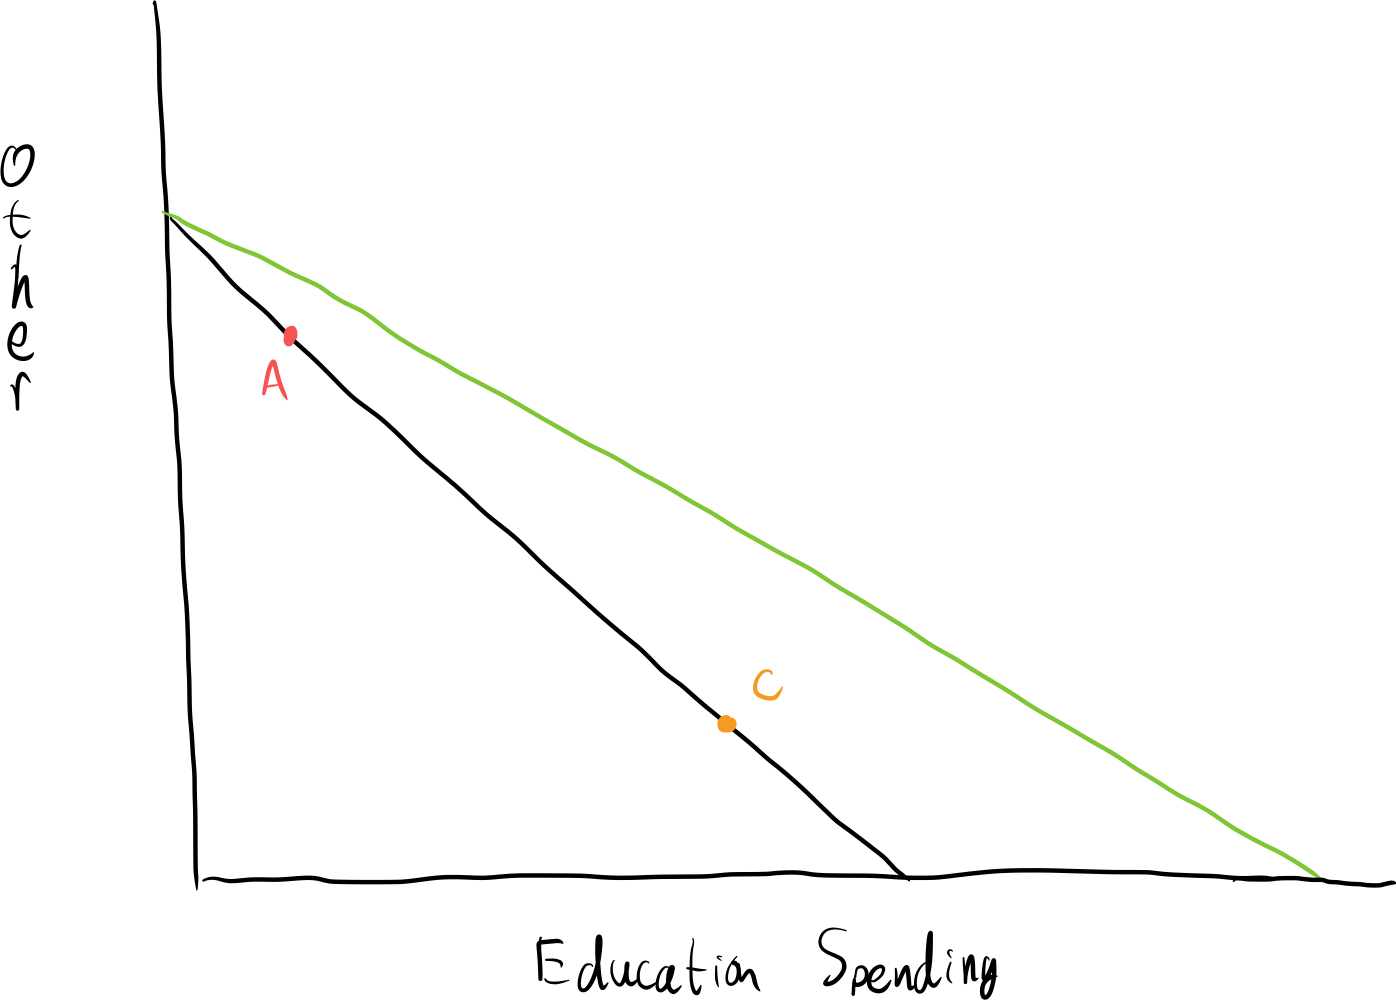
\includegraphics[width=10cm]{images/matching_grant.png}
          \end{center}
          The matching grant is most likely to increase relative education spending of all the classes of grants.
      \end{itemize}
      \item[Grants In Practice:]\hfill
        \begin{itemize}
          \item Foundation grant: states guarantee minimum level of funding (restricted block grant).
          \item Power equalization grant: states subsidize tax revenue for low-income areas (matching grant).
          \item Equalization grant: direct aid on the basis of wealth (unrestricted block grant).
          \item Centralization: 100\% state funding.
        \end{itemize}
    \item[Foundational Grant: Deep Dive] Let $B_{d} = W_{d}\tau_d$. Then, the grant to $d$ is denoted $G_d = \max\{0,F - (\tau^{F}W_d)\}$, where $F$ is the foundation level and $\tau^{F}$ is the foundation rate. If the wealth of the district is less than the foundation level, the government will grant money to make up the difference.\\

      Wealthy districts will not be affected by the foundation grant (as their endowment exceeds the foundation level).\\

      In theory, the foundation grant could tax away from rich districts to distribute toward poorer districts --- this would prompt wealthy districts to reduce their tax rates until they reach the foundation level, and likely decrease overall education spending.\\

      Politically speaking, centralization and equalization of funding tends to be impossible (and it's not clear that it's desirable to have fully equal spending). Perverse effect of school funding equalization tends to be lower total education spending.\\

      However, grants tend to reduce inequality --- but not by much.
  \end{description}
  \subsection{Tiebout Sorting}%
  \begin{description}
    \item[Overview:] People will move to areas that reflect their preferences for education (or any public service). Local governments are competing with each other.
    \item[Why Local Governments?] There are multiple reasons for local government-provided public education
      \begin{itemize}
        \item Transportation
        \item Grade consistency
        \item No credit constraints
        \item Economies of scale (in special education or athletics)
      \end{itemize}
    \item[Why Taxes?] Suppose there was publicly provided education, but financing was voluntary. However, this brings a free-rider problem (the Nash equilibrium of public goods spending is lower than the optimal quantity of public goods spending).
    \item[Tiebout Sorting:] Assuming a large metropolitan area with a high quantity of districts, similar housing stock, high mobility, and elastic funding, people will ``vote with their feet'' to the district with their preferred public goods spending. Housing prices serve as the market clearing mechanism.
    \item[Consequences of the Tiebout Model:]\hfill
      \begin{itemize}
        \item There is no need to ask people's willingness to spend, as their preferences are revealed through migration.
        \item Allocative efficiency: consumers live where services match their preferences.
        \item Productive efficiency: local governments produce services at a rate to match population preferences.
      \end{itemize}
    \item[Challenges:]\hfill
      \begin{itemize}
        \item Mobility is often limited.
        \item Consumers are often not fully informed.
        \item There are often not a lot of options.
        \item Assumption of fully local return (absence of spillovers).
        \item Assumption of zero resource constraints.
        \item Property taxation.
        \item Reflects preferences of parents over children.
      \end{itemize}
    \item[Evidence for Tiebout Sorting:]\hfill
      \begin{itemize}
        \item Schooling is often a large part of choice of residence.
        \item Hedonic model suggests yes.
        \item The next question is whether or not competition between schools increases academic achievement.
        \item Hoxby (2000) suggests that Tiebout sorting improves educational outcomes.
      \end{itemize}
  \end{description}
  \section{Lori L. Taylor: Government's Role in Primary and Secondary Education}%
  \begin{itemize}
    \item Migration through high schools --- what happens after? Brain drain: people who get educated in a community leave for a different location.
    \item In-migration of educated people has a tendency to yield \textit{decreased} education spending; while the questions in the paper are still relevant, the paper still deals with data limitations.
    \item Rationales for government spending:
      \begin{itemize}
        \item Market failure.
        \item Externalities.
        \item Altruism.
        \item Alternatives: cultivating virtues.
      \end{itemize}
    \item Paper takes for granted that there is a private return to education. The question is whether or not the government should be involved.
    \item Second-best externalities as a rationale: higher education leads to higher incomes, which leads to higher tax revenue and amenities. If the marginal tax dollar is a positive return, and education has a positive return on taxes spent, then private returns to education do not reflect social returns.
    \item First-best externalities: spillovers lead to higher productivity, reduction in crime (since you're preoccupied with school). However, education outside of its role as preoccupation does not indicate that education has benefits.
    \item Corrective policies:
      \begin{itemize}
        \item Market failure: ensure that financing options for education are of similar price to other forms of loans.
        \item Externalities: the government should subsidize education proportional to the size of the externality. Since the private return to education is high, suggests that most of the payment for education should fall on parents.
        \item Altruism: society should transfer resources, but does not imply that the government should operate education.
      \end{itemize}
    \item Benefit to public education vs. access to education.
      \begin{itemize}
        \item Currently, education access is based around public school districts.
        \item Alternative may include voucherization: every school has a price, give every child a voucher for reimbursement of certain amount of cash. Potentially more efficient.
        \item Voucherization leads to the question of how much power should parents have over their children's education.
      \end{itemize}
    \item Parental involvement in (primary and secondary) education:
      \begin{itemize}
        \item In favor: it's very hard to make an argument against parental control without it spiraling into a lot of authoritarianism.
        \item Implication is not in favor of tax-supported, government-run public education.
        \item However, there are a lot of arguments against the idea of near-full parental control over children's education.
      \end{itemize}
    \item Potential outcomes framework:
      \begin{itemize}
        \item There's a lot of stuff that we're doing today that is mostly due to path dependence. It's nearly impossible to imagine a world without a lot of public education.
        \item This paper brings the argument that core economic arguments do not necessarily lead you to the model of education that we have today.
      \end{itemize}
  \end{itemize}

  \section{Primary Education Policy}%
  Consider some of the inputs of the education production function:
  \begin{itemize}
    \item Textbooks;
    \item Teachers;
    \item Infrastructure;
    \item Student Funding;
    \item Class size;
    \item Computers;
    \item Community;
    \item Greenery;
  \end{itemize}
  We can see that a lot of these inputs ultimately come down to school funding.\\

  Primary question: does funding schools better matter --- however, there is a large endogeneity problem when simply regressing educational outcomes vs. school funding. Once we are able to remove this endogeneity problem, our question is now between the different methods of spending.
  \begin{description}
    \item[Rosenwald Schools:] Philanthropic initiative, built 5000 schools in various counties around the United States south built using using matching grants. Some counties got multiple new schools, others got 1 or 0 new schools.\\

      Treatment group saw literacy grow faster: 6\% increase in literacy above and beyond the counterfactual (particularly beneficial for Black students).
    \item[Card and Krueger (1996):] Compared North and South Carolina --- little differences in characteristics of Black population in states, but had different economies. North Carolina was dependent on tobacco (less labor-intensive, easy to mechanize) while South Carolina was dependent on cotton (labor-intensive). Emphasis on education in South Carolina for Black students was lower than in North Carolina --- North Carolina had bad schools, but South Carolina had worse schools.\\

      The average class size for Black students in South Carolina was substantially higher than in North Carolina. However, around 1920, there is a large convergence of school funding and class sizes start converging too.\\

      Card and Krueger compare outcomes for Black students in NC vs. SC (with White students as a control), as quasi-experimental in returns to student funding.\\
      
      Card and Krueger found that the decline in class sizes increased relative wages by 6\%. Takeaway: class sizes matter.
    \item[Green and Hofmann (1965):] Prince William County, Virginia closed all public schools from 1959--1963.
    \item[Primary Takeaways:] Increasing funding tends to yield positive educational outcomes. However, there is actually mixed evidence.
    \item[Trends in Data:] School spending has increased about 10x since 1940 to today, salaries are up 45\% in real terms, and student:teacher ratios are down 44\%. However, despite this increase in school resources, NAEP scores have not increased all that much.\\

      We see that states that spend more have more educated populations and better outcomes, but increased spending over time does not predict a change in outcomes. Effectively, the places with better education outcomes demand higher education spending, but that does not imply that increasing education funding helps increase education outcomes.
  \end{description}
  \section{Caroline M. Hoxby: Does Competition Among Public Schools Benefit Students and Taxpayers?}%
  \begin{itemize}
    \item Good empirical work requires data expertise. A simple model like $A_i = \beta_0 + \beta_iC_i$ will be affected by so many elements in the potential outcomes framework.
    \item Broadly speaking, choice increases education productivity.
    \item However, the instrumental variable chosen does not necessarily allow for full predictive power, ultimate results are based on very few metropolitan areas.
  \end{itemize}
  \section{Teachers: Education Production Function and Labor Market}%
  \begin{description}
    \item[Measuring Teacher Impact:] Teachers are probably the most important input into the education production function; we may be curious as to how to measure quality.
      \begin{itemize}
        \item The value-add model uses quantitative measurements to see how students' results grow as a result of the teacher's teaching.
        \item Policy has a tendency to focus on short-run value add (via test scores, for instance).
        \item However, test scores do happen to correlate well with other measures we tend to care about (e.g., graduation rates, incomes).
      \end{itemize}
      There are some particular issues with the teacher value-add model:
      \begin{itemize}
        \item Mobility
        \item Selection Bias
        \item Small $N$, teacher turnover
      \end{itemize}
      We can also use a Bayesian approach (from Chetty 2014).
      \begin{align*}
        \theta_{j}^{\ast} &= \tau \overline{Y_{j}} + (1-\tau)\mu_{\theta},\\
        \tau &= \frac{\sigma_{\theta}^2}{\sigma_{\theta}^{2} + \sigma_{\epsilon}^{2}/N}
      \end{align*}
      where $\theta_{j}^{\ast}$ is teacher quality, $\overline{Y}_j$ is test scores, and $\mu_{\theta}$ is the teacher value add, and $\sigma_{\epsilon}^2$ denotes the variance of students' test scores. Essentially, as classes become large, $\tau \rightarrow 1$ and teacher quality is more predicted by test scores.
    \item[Evidence for Teacher Impact:] From Rivkin, Hanushek, and Kain (2005), Rockoff (2004), and Chetty et al. (2014), we find:
      \begin{itemize}
        \item A 1 st. dev. improvement in teacher quality increases test scores by 0.1 standard deviations.
        \item A 1 st. dev. deviation improvement in teacher quality is equivalent to reducing class size by 10 students.
        \item A 1 st. dev. teacher improvement does not fade, increasing college going by 0.5\% and earnings by 0.09\%.
        \item The NPV for 1 year of education at 1 st. dev. above mean is \$115,000.
      \end{itemize}
      From this evidence, we can see that teachers do matter. However, we don't know how to predict teacher quality. There is some correlational evidence.
      \begin{itemize}
        \item Experience above 6 years tends to lead to improved outcomes (but there is obviously survivorship and selection bias)
        \item There is no evidence that credentialing or degrees matter.
        \item There is limited role model evidence (e.g., Teach For America leads to small, increased college applications, but not increased college going, increased chance of women majoring in STEM if their intro track professors are women). However, taking the role model evidence to its full extent leads to full segregation, which wholly unactionable.
      \end{itemize}
    \item[Teacher Labor Market:] Wages are the price of labor, supply is teachers and demand is students and administration.
      \begin{itemize}
        \item Increased population, smaller class size, district resources, and school choice all can affect demand for teachers.
        \item Outside options, working conditions, salary structures, and credentialing rules all can affect the supply of teachers.
      \end{itemize}
    \item[The Roy Model:] Understanding teacher supply based on skills and outside options. 
      \begin{itemize}
        \item Skill collapsed into one dimension, $s$.
        \item Potential teachers live in one period.
        \item Teachers choose the profession that yields the highest lifetime income.
        \item Teaching has wage structure $w_T= \alpha_T + \beta_T s$ and other careers has wage structure $w_O = \alpha_O + \beta_O s$
      \end{itemize}
      \begin{center}
        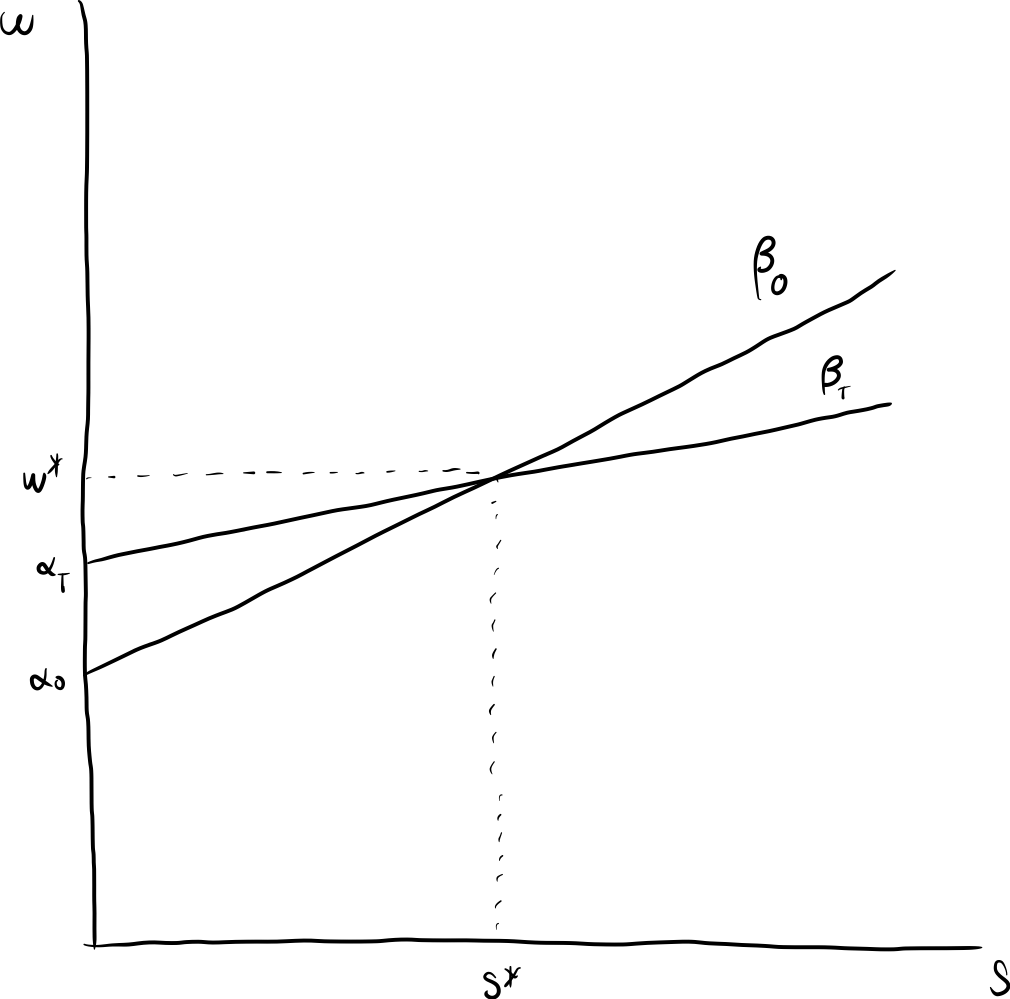
\includegraphics[width=7.5cm]{images/returns_to_skill_teachers.png}
      \end{center}
      We can see some potential changes in the $w$/$s$ relationship.
      \begin{itemize}
        \item Alternative labor market options increase $\alpha_O$ for people at all skill levels and increase $\beta_0$.
        \item Teacher unionization compresses the wage scale, meaning $s$ is not rewarded as much, so $\beta_T$ reduces.
      \end{itemize}
    \item[Empirical Results:]\hfill
      \begin{itemize}
        \item There has been a substantial increase in teacher unionization (including Meet and Confer provisions and collective bargaining contracts) from the 1960s to the current era.
        \item There has also been a large increase in the proportion of women in other educated professions (such as medicine and law).
        \item In alignment with these trends, there has been a reduction in teacher aptitude relative to the college graduate population.
        \item However, despite the relative reduction in teacher aptitude, NAEP scores have been stagnant for White Americans and have actually increased for African-Americans (contrary to the expectation that they would reduce).
        \item There are many potential sources of this trend not related to teachers, such as environmental improvements.
      \end{itemize}
  \end{description}
  \section{Carrell and West: Does Professor Quality Matter?}%
  \begin{itemize}
    \item Teaching to the test: experience both from the paper and personal high-stakes testing experience suggests that it may be detrimental.
    \item There is evidence that teachers would be better off knowing \textit{less} about the standardized tests.
    \item Causality is much stronger in the Air Force Academy due to randomization; however, selection in non-random assignment of classes suggests the effects may go in either direction.
    \item From the paper, we can answer the question of teachers mattering (yes), but that good teachers may not be the ones who have the best contemporaneous value-add.
  \end{itemize}
  \section{School Accountability}%
  \begin{itemize}
    \item Principal-agent problem: government wants to increase educational performance, incentives can be implemented at different levels.
      \begin{itemize}
        \item School accountability: rewards and punishments at the school level.
        \item Teacher accountability: rewards and punishments for teachers.
        \item Student accountability: rewards and punishments for students.
      \end{itemize}
    \item Potential outcomes to incentivize:
      \begin{itemize}
        \item Expected future earnings.
        \item College acceptance rate.
        \item Standardized test scores.
      \end{itemize}
      If the focus is on standardized test scores, the most likely lever to be effective is at the school level.
    \item We looked at teacher quality last time, where we saw that teachers vary in quality and they affect their students' outcomes. However, teachers are often subject to a rigid pay scale (and said rigid pay scale is often part of the appeal of teaching).
    \item Proposals for merit-based pay are based in the idea that tying teachers' salary to education productivity provides an incentive for increasing education productivity.
    \item The primary measure of education productivity is standardized test scores.
    \item Tennessee merit pay program:
      \begin{itemize}
        \item Five pay stages not based on test scores --- principal, peer, and external evaluations.
        \item Teachers could opt in or opt out.
        \item The treatment was not randomly assigned --- comparing teachers who chose to opt in vs. those who did not would yield a biased estimate of the effect of merit pay.
        \item Dee and Keys (2005) used data from Project STAR, which randomly assigned students and teachers to classes of different sizes (and vice versa). They were able to make across-classroom comparisons within the same school.
        \item They found that merit pay was associated with statistically significant gains in math test scores.
        \item Merit pay improved for both beginner teachers and experienced ones too.
      \end{itemize}
    \item Many states had merit pay programs in the 1980s, but by 2008 only 8 states had some form of teacher merit pay.
    \item Teach for America:
      \begin{itemize}
        \item Program that provides a ``fast track'' for teacher certification, two year commitment to the program, with no requirement for a particular degree.
        \item Lowers the cost of entering the teaching profession, and the marginal teacher is more highly skilled (by the Roy model).
        \item Raymond and Fletcher (2000) took a sample of non-TFA and TFA teachers from Houston, and compared student test score gains (controlling for other factors influencing teacher type).
        \item They found that TFA teachers were no worse than non-TFA teachers, and TFA teachers were associated with significant gains in math scores. TFA teachers also had lower variance in the distribution of their outcomes.
        \item New TFA teachers were much stronger than new non-TFA teachers, but those relative gains are temporary compared to all other teachers.
        \item However, as TFA expanded, the marginal hire became less skilled --- and competition for TFA teachers became stronger.
      \end{itemize}
    \item Features of school accountability programs:
      \begin{itemize}
        \item Student achievement (typically measured by standardized test scores).
        \item Public reporting of school performance.
        \item Rewards or sanctions based on performance.
      \end{itemize}
    \item Federal No Child Left Behind Act passed in 2001, and public reporting laws spread in the late 1990s, growing from 5 states to 45 by 2002.
    \item Accountability measures generally required that children in grades 3--8 be tested, focused on mathematics and English reading.
    \item Sanction for underperformance usually resulted in vouchers for parents of students, schools reconstituted as charters, or administration replaced.
    \item Why accountability might not work:
      \begin{itemize}
        \item Test scores are noisy measures (variation in test scores is often random).
        \item We want to know the value of $V(\varepsilon)/V(y^{\ast})$.
        \item We can measure in three ways: levels, changes (across cohorts), gains (within cohort).
        \item Concerns include school size --- we see that test scores become more clustered around the mean at larger schools than smaller schools. Small schools thus have more noise to them. The Bill and Melinda Gates foundation famously had to course-correct regarding school size after mistaking this noise for causation.
        \item We see that levels have the least noise, gains have the second least noise, and changes have the largest noise.
        \item Using test score gains requires lots of data, and we should avoid drawing strong inferences from single-year changes.
      \end{itemize}
    \item Jacob (2003) found that there was better student performance, but there was also a rise in special education, more non-participation and non-reporting bias, implying that schools did change behavior.
    \item Figlio and Winicki (2002) found that there was an increase in average calories for school lunches in underperforming districts during testing weeks (versus non-underperforming districts). This is a potential mechanism for increased test scores.
  \end{itemize}
  \section{Dee and Jacob: The Impact of No Child Left Behind}%
  \begin{itemize}
    \item NCLB was probably the longest-lasting education reform, so there is more evidence for its effects than other federal school accountability measures.
    \item Paper finds robust benefits for fourth grade math (via NAEP scores) from NCLB.
    \item NCLB also improved math scores especially for Black and Hispanic students.
    \item However, improvement in reading scores was not statistically significant.
  \end{itemize}
  \section{School Choice and Peer Effects}%
  \begin{itemize}
    \item Broadly speaking, there are two methods to ``do'' school choice.
      \begin{itemize}
        \item Vouchers: funding for schools follows the student.
        \item Charter Schools: publicly-funded, privately-operated schools. Generally operated via lottery admissions with pupil-based funding. Grew in popularity during the 2000s and 2010s.
      \end{itemize}
    \item Traditional model is generally neighborhood-dependent (your address is zoned for a particular school that you go to). Almost every school district has some mechanism to allow students to attend schools that aren't the neighborhood school.
    \item We can view charter schools as creating competition in the education market (as opposed to the current model of local public school monopolies). The marginal benefit to charter schools tends to decrease as their quantity increases.
    \item Question: would you rather attend Occidental with La Verne students or attend La Verne with Occidental students?
    \item The answer to the question ``do your classmates matter?'' is generally ``yes,'' but there are lots of endogenous effects.
    \item Manski (1993) posits that social effects are important.
      \begin{align*}
        Y_{ig} &= \beta_0 + \beta_1 \overline{Y}_{-ig} + \beta_2\overline{X}_{-ig} + \beta_3X_i + \delta_g + \varepsilon
      \end{align*}
      Essentially, we say that your outcomes are a function of the outcomes of your peers, as well as $X$, or background characteristics of your peers and yourself.\\

      However, it's hard to exactly pin down why peers matter. We call $\beta_1$ the endogenous parameter (or effort effect) and $\beta_2$ the exogenous parameter (or contextual effect).\\

      We can see that the model is decent at describing the world, but it can never actually be run. There is a large problem of reverse causality --- if your friends affect you, then you affect your friends.\\

      We should care about peers, but it's very hard to understand their effects.
    \item Hoxby (2000) studies the question in primary school, while Sacerdote (2000) studies the question at college. Both try to find a way to overcome the endogeneity problem.
    \item Sacerdote uses random assignment of roommates to obtain his results.
    \item Genealogy of Peer Effects Literature:
      \begin{itemize}
        \item Manski (1993): peer effects are important, but hard due to reflection, selection, and endogenous sorting.
        \item Hoxby (2000) and Sacerdote (2000) study contextual effects and effort effects.
        \item Sacerdote uses random roommate assignments, shows presence of some peer effects. However, Sacerdote cannot break apart contextual vs. effort effects.
        \item Hoxby looks at multiple years of data from a large group --- variance on gender, race, and socioeconomic status (free or reduced lunch eligibility). Classrooms with lots of girls tend to have better educational outcomes for everyone (including boys).
        \item Carrell (2002) takes a similar approach to Hoxby, and links domestic violence to peer achievement.
        \item Once economists settled on a model that they're convinced gives credible results, Brown (2004) uses it for golf.
        \item Ross (2008) uses an instrumental variable for high school peer effects to separate $\beta_1$ and $\beta_2$. They're able to find that both exist.
        \item Carrell et al. (2008) uses USAFA data to find non-linear peer effects. Up until this paper, we don't know whether peer effects are welfare-improving. They find that peer effects exist for some students and not for others --- bottom tercile students benefit from high SAT-verbal score peers.
        \item Carrell et al. (2013) run a controlled experiment based on Carrell et al. (2008) by designing optimal peer groups.
      \end{itemize}
    \item One of the newer approaches is a focus on the effects of variance in peers, as well as social networks (calculated using an adjacency matrix).
    \item Other measures of peer effects are focused on homophily (i.e., people tend to associate with similar people). Currani, Jackson, and Pin (2009) take a baseline of $0$ for random friendships, and find that particular racial groups befriend each other at a rate above random. Specifically, they find that homophily peaks around 40--50\% of the population.
      \begin{itemize}
        \item Most predictive is gender, second-most predictive is race, and third most-predictive is academic ability.
        \item In the Carrell experiment paper, we could see that there was more clustering. 
      \end{itemize}
    \item Measuring peer effects from social networks is likely to bring even more endogeneity, but improves our assumptions.
    \item Sharing ideas is effectively free --- rates of sharing ideas, however, requires more friends. Students with similar levels of academic aptitude tend to share more ideas and do better as a result. 
  \end{itemize}
  \section{Derek Neal: How Vouchers Could Change the Market for Education}%
  \begin{itemize}
    \item Parents care a lot about the institution as well as the peers --- under voucherization, we may wonder what parents might value. 
    \item Efficiency of vouchers relative to Tiebout sorting vs. geography.
      \begin{itemize}
        \item Practicality: if low-income families are given vouchers, would they be able to afford private schools or would private schools have to subsidize tuition? Idea would be that religious schools (or schools run like religious schools) would be more affordable.
        \item Elasticity of demand: certain private schools have very inelastic demand.
        \item Vouchers would reduce the location value of wealthy neighborhoods. However, in urban areas where options are higher and transportation costs are lower, it's likely that vouchers would increase the value of such locations.
      \end{itemize}
    \item Vouchers might increase sorting. Increasing heterogeneity of education increases variance, including the possibility of very high costs.
      \begin{itemize}
        \item Benefit of sorting: broadening the base of demand could provide more specialized education relative to the current system.
        \item Downside of sorting: very few barriers to creating a school with very high social costs (à la the ``Eastside Ku Klux Klan Academy''). 
      \end{itemize}
  \end{itemize}
  \section{Carrell, Sacerdote, and West: From Natural Variation to Optimal Policy? The Importance of Endogenous Peer Group Formation}%
  \begin{itemize}
    \item External validity: variance in the AFA is much likely to be smaller than the average high school (or even many colleges). The AFA is already effectively tracked --- it has high admission standards.
    \item The tracking in the paper is much more hyper-local than tracking in a typical high school.
    \item Cliques often form due to similar interests/circumstances. We would expect that dedication at the AFA is higher than at a typical high school, so the peer effects might be muted.
    \item At the AFA, there is more contact with peers than at a typical high school or college, so the peer effects may be increased.
    \item Randomized experiment in an external setting yielded some peer group formations between people of higher relative ability and lower relative ability.
    \item Experiment setup had control group (with squadrons randomized on the basis of ability), and treatment groups (one of a large number of top and bottom tercile students, and one of a large number of middle tercile students).
    \item Middle tercile group found significant positive effects, but in treatment group with large number of top and bottom tercile students, bottom tercile students had worse results.
    \item It is likely that top tercile students are largely unaffected by peer effects --- self-drive tends to be higher. Additionally, measurable achievement is capped --- it's effectively impossible to go past a 4.0. It is possible that the intervention reduced their abilities, but they were above the cutoff nonetheless.
  \end{itemize}
  \section{The Market for Higher Education}%
  \begin{itemize}
    \item Modern universities can largely be traced back to the University of Bologna (1088) and Oxford University (1096).
    \item Before the 1800s, the structure of higher education was largely focused on teaching rather than research --- lots of education was focused on preparing people to be priests.
    \item In 1776, there were 18 universities, total enrollment of around 750.
    \item Clark (2014) found that ancestors attending early universities predicted wealth today.
    \item Goldin and Katz (1999) find that higher education starts to take off in the late 19th century, as demand for scientific research and technical knowledge increased with the rise of industrialization.
    \item With the passage of the G.I. Bill in 1944, many more veterans start to attend higher education, coinciding with the entrenchment of state higher education systems (such as the University of California).
    \item During the Cold War, demand for scientific research grew significantly, and the modern university comes into its own during this period. Women also start entering the sciences as their labor market options expand dramatically.
    \item At a macro-level, not much has changed from the 1980s to present (in terms of the style and quality of higher education). Enrollment has largely plateaued (due to demographic shifts). There is a lower level of state support for higher education, in part because people will pay a lot of money for higher education.
    \item There is much heterogeneity and stratification in higher education.
      \begin{itemize}
        \item Chicago has 83 four-year universities, with over 100 private two-year institutions.
        \item The University of Chicago spends upwards of \$60K/student/year.
        \item There are 5 four-year public institutions in Chicago with a total of 60K students.
        \item There are 22 two-year public universities, which expend less than \$3,000 per student per year.
        \item Heterogeneity refers to the offerings in the higher education market.
        \item Stratification tends to refer to the rankings/differences by grouping of higher education.
      \end{itemize}
    \item Higher education is a customer input technology --- inputs are the outputs, and (selective) higher education rival.
    \item Higher education is also a mixed market --- there are private and public options with not-for-profit and for-profit segments in private education.
    \item The primary market failure in higher education is \textit{asymmetric information}.
      \begin{itemize}
        \item Finances (primarily apply to higher education).
        \item Faculty and major quality, as well as student opportunity.
        \item Peers.
        \item Alumni.
        \item Spending per student.
        \item Future plans.
      \end{itemize}
      Asymmetric information leads to principal-agent problems; schools do not have the same incentives as students in achieving a goal.
    \item Marginal cost of higher education tends to decrease as enrollment increases --- large public institutions tend to educate students at a much lower cost per student.
    \item Higher education also has economies of scope --- efficiencies in increasing variety of educational offerings. Pretty much no college offers a major in only one course of study, as opposed to private industries that feature extreme specialization.
      \begin{itemize}
        \item Increase diversity and obtain a larger demographic of students.
        \item Major shopping and uncertainty.
        \item Common needs --- registration systems, grant administration, etc.
      \end{itemize}
    \item The government serves many roles in higher education.
      \begin{itemize}
        \item Appropriations --- primarily at the state level.
        \item Financial aid (directly to students) --- 90\% federal, 10\% state.
        \item Research funds, through the NSF and NIH.
        \item Land grants --- public universities do not pay rent or property taxes on their land.
        \item Not-for-profit status is often provided to institutions of higher education, exempting their earnings from taxation.
      \end{itemize}
    \item Public institutions tend to get more money from the state (and less from endowments), while private schools reverse this order.
      \begin{itemize}
        \item Endowments tend to withdraw approximately 5\% of the endowment per year to use in their annual budget --- endowments can grow about 5\% YoY, so the endowment can be maintained. (Author's note: asset managers are thieves, I get 7\% YoY on my Vanguard account and I'm not charge 1\% AUM.)
        \item If the state drops funding by \$1, then endowment needs to increase by \$20 to make up the budget loss.
        \item States have been pulling back on higher education spending over the last 50 years, meaning endowments tend to need to grow even faster. As a result, tuition tends to increase.
      \end{itemize}
  \end{itemize}
  \section{The Cost Disease in Higher Education}%
  \begin{itemize}
    \item Hoxby discusses MOOCs as a way to ``standardize'' non-selective education, vs. the investment style of education inherent in selective colleges. One probably wouldn't expect particularly strong cost reductions beyond a certain point, due to the other factors driving people towards college educations (especially at liberal arts colleges), such as personal interaction with other students and professors.
    \item ``Buying the best:'' amenity creep (colleges will better recruit students when they offer better amenities), pressure to increase teacher-student interaction opportunities, offering more and more merit aid, etc. all contribute to costs spiraling upward.\\

      Recall that all the inputs to the education production function tend to correlate with income --- merit aid systems tend to privilege wealthier students. Desire to increase prestige of student population yields increased costs for providing aid to people who do not necessarily need it.
    \item Average student pays around 54\% of total tuition cost. If a college wants to increase its budget by \$1, the college effectively needs to increase its tuition by \$1.87.
    \item Federal student loans have an interest rate lower than the market interest rate --- students are able to afford a larger loan package from a federal loan than from a private loan. Since funding is effectively guaranteed, schools can increase their prices further. Schools capture a large proportion of the subsidy.
    \item Baumol's cost disease: Mozart's String Quartet will always require four people --- certain things require a certain amount of labor or time regardless of technological improvements. Higher education is generally quite resistant to productivity improvements. Professors are effectively paid to force us to spend more time learning a topic.
    \item There is a lot of resistance to change in higher education --- even if offering PhD programs is inefficient relative to postdocs, or maintaining the tenure system relative to mandatory retirement is inefficient, schools still keep them in place.
    \item The wage structure of faculty tends not to be set by productivity (relative to typical private industries). Wages tend to be set on the basis of alternatives --- general economic growth outside academia yields growth in faculty wages.
    \item There are a host of downsides to hybrid learning --- it's often harder to learn with hybrid learning, with less flexibility and an often bad learning environment. Additionally, in-person education consists of dedicated time --- reduces procrastination.
    \item Potential methods to reduce inequality between institutions --- changing endowment system, increasing progressivity of education subsidies.
  \end{itemize}
\end{document}
